\chapter{}

\section{Pruebas}

\subsection{Prueba despliegue}

Para probar la creación de la máquina virtual en Amazon AWS vamos a mostrar el resultados de ejecutar el Vagrantfile mostrado anteriomente. Es necesario ejecutar la orden \texttt{vagrant up --provider=aws}:
\begin{figure}[H] %con el [H] le obligamos a situar aquí la figura
\centering
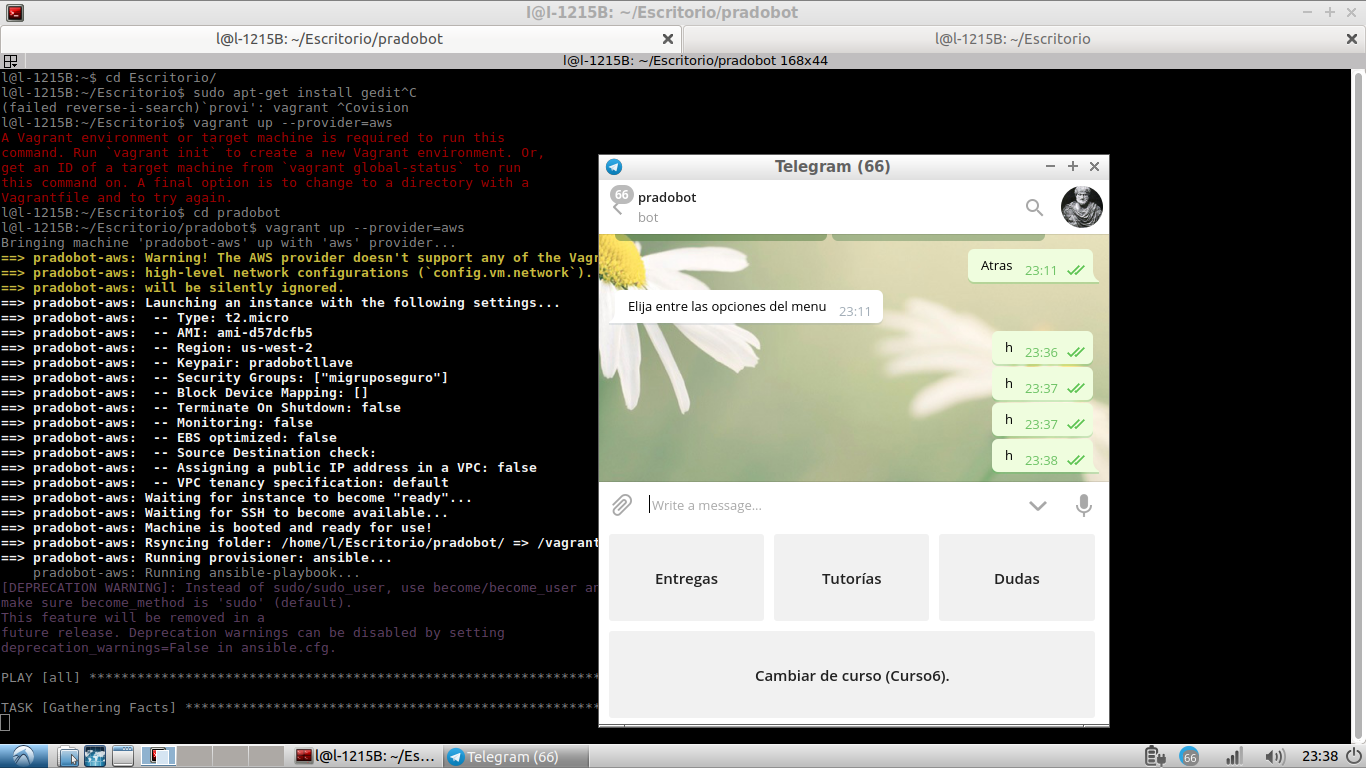
\includegraphics[scale=0.3]{imagenes/random/123bot.png}  %el parámetro scale permite agrandar o achicar la imagen. En el nombre de archivo puede especificar directorios

\caption{Ejecutando los tests de la aplicación}\label{figura92}

\end{figure}

En la salida de la orden se pueden ver las características de la máquina virtual creada tras lo cual una vez está habilitado ssh se ejecuta el playbook de Ansible:

\begin{figure}[H] %con el [H] le obligamos a situar aquí la figura
\centering
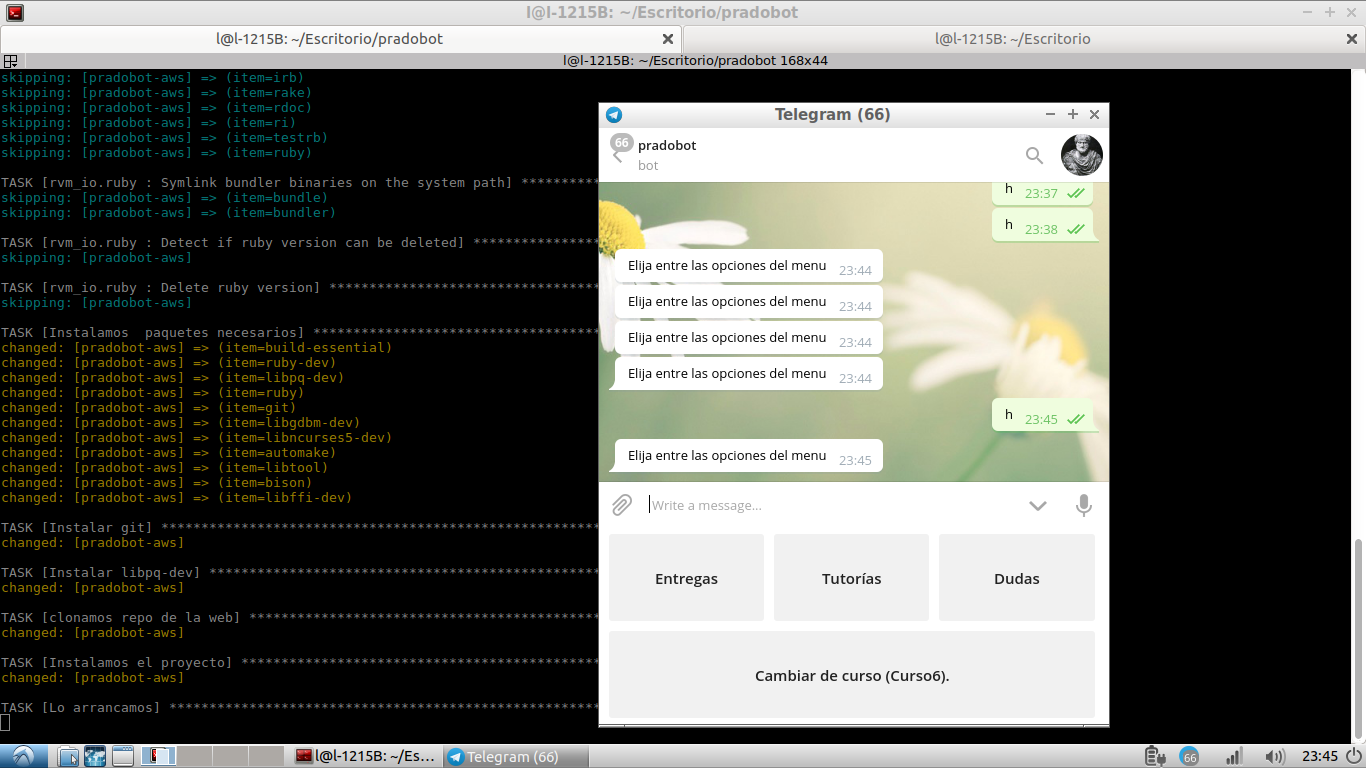
\includegraphics[scale=0.3]{imagenes/random/123bot2.png}  %el parámetro scale permite agrandar o achicar la imagen. En el nombre de archivo puede especificar directorios

\caption{Finalización de aprovisonamiento con Ansible}\label{figura94}

\end{figure}

La última tarea del playbook de Ansible lo deja ejecutándose. Por falta de tiempo no se ha podido configurar Ansible para que despligue el proceso y asi no se quede pillado en la terminal y configurar adicionalmente una herramienta adicional que iniciara y parara la ejecución de pradobot en la máquina virtual cuando se deseara.



\subsection{Tests}

Para ejecutar los tests unitarios que componen la aplicación es necesario ejecutar la orden \texttt{rake} en el directorio en el cual se encuentra el Rakefile. Esto hará que rake lea los ficheros especificados en el Rakefile y ejecute los tests contenidos en ellos uno a uno:

\begin{figure}[H] %con el [H] le obligamos a situar aquí la figura
\centering
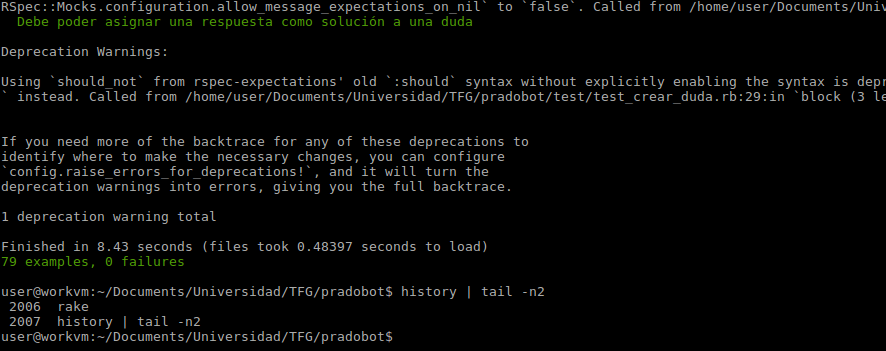
\includegraphics[scale=0.4]{imagenes/random/Screenshot_2017-08-30_16-40-12.png}  %el parámetro scale permite agrandar o achicar la imagen. En el nombre de archivo puede especificar directorios

\caption{Ejecutando los tests de la aplicación}\label{figura92}

\end{figure}

Como podemos ver en la imagen superior se muestra en verde cada test que ha pasado satisfactoriamente dando al final un resumen del número de tests ejecutados (79 examples) y de cuántos han fallado (0 failures) indicando además cuánto tiempo se han tardado en ejecutar los tests.
\par
En caso de fallo en algún test se muestran al final las razones por las que han fallado los tests en rojo.

\begin{figure}[H] %con el [H] le obligamos a situar aquí la figura
\centering
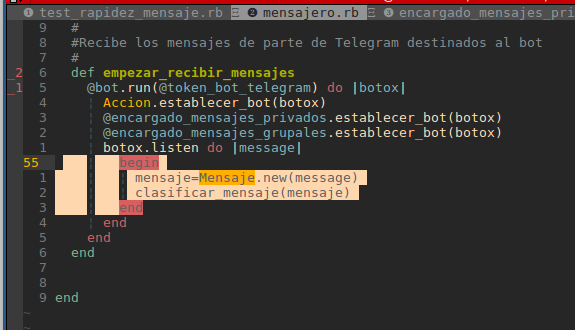
\includegraphics[scale=0.6]{imagenes/random/Screenshot_2017-08-27_11-49-39.png}  %el parámetro scale permite agrandar o achicar la imagen. En el nombre de archivo puede especificar directorios

\caption{Tras ejecutarse los tests se muestran los que dan fallo}\label{figura94}

\end{figure}

\subsection{Rendimiento}
Realizar test de rendimiento sobre el programa es complejo, ya que cualquier mensaje que se le mande al bot implicará llamadas a la base de datos y hacer mocks y stubs solamente es práctico si se va ha realizar un test sobre una parte del sistema. Aún así vamos a probar a mandar varios mensajes desde chats privados y grupales midiendo el tiempo que se tarda en procesar los mensajes. El código utilizado en la medición es el siguiente:
\begin{figure}[H] %con el [H] le obligamos a situar aquí la figura
\centering
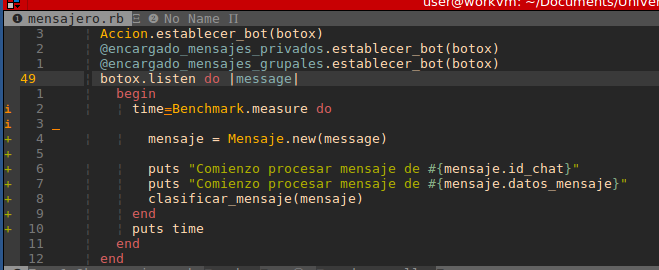
\includegraphics[scale=0.6]{imagenes/random/rend1.png}  %el parámetro scale permite agrandar o achicar la imagen. En el nombre de archivo puede especificar directorios
\caption{Código utilizado para la medición del tiempo que se tarda en procesar un mensaje}\label{figura94}
\end{figure}



Se ha utilizado la función \texttt{measure} del módulo de benchmarking de ruby \href{https://ruby-doc.org/stdlib-2.0.0/libdoc/benchmark/rdoc/Benchmark.html}{Benchmark}. Esta imprime el tiempo de CPU en espacio de usuario (\textit{ CPU time}), tiempo en el kernel realizando operaciones para nuestro programa (\textit{system CPU time}), la suma de los dos  y después el tiempo que se ha empleado en total (\textit{elapsed real time}). Los tiempos obtenidos son los siguientes:

\begin{figure}[H] %con el [H] le obligamos a situar aquí la figura
\centering
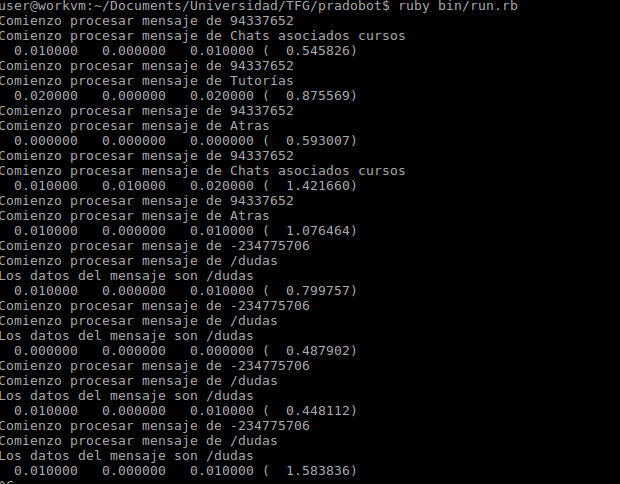
\includegraphics[scale=0.6]{imagenes/random/rend2.png}  %el parámetro scale permite agrandar o achicar la imagen. En el nombre de archivo puede especificar directorios
\caption{Tiempo que tarda pradobot en procesar mensajes procedentes de un chat privado y de unchat grupal}\label{figura94}
\end{figure}

Como podemos observar los tiempos de CPU suelen rondar los 0.1 segundos, mientras que el tiempo real empleado es de entre 0.8-2 segundos. Esta diferencia es bastante significativa. Vamos a probar a mandar mensajes con otro programa  \enquote*{telegram-cli}. Este programa permite mandar mensajes a un chat de Telegram desde la terminal:


\begin{figure}[H] %con el [H] le obligamos a situar aquí la figura
\centering
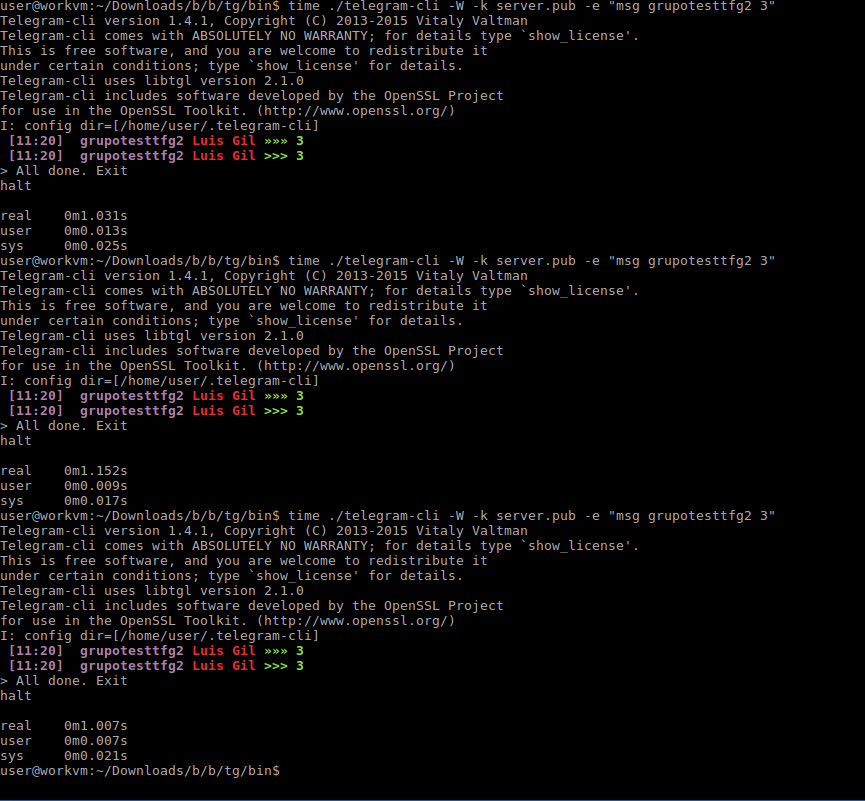
\includegraphics[scale=0.4]{imagenes/random/Screenshot_2017-09-01_11-21-38}  %el parámetro scale permite agrandar o achicar la imagen. En el nombre de archivo puede especificar directorios
\caption{Envío de mensaje utilizando telegram-cli}\label{figura94}
\end{figure}

Como se puede apreciar la diferencia de tiempo entre el tiempo de CPU total y el tiempo real sigue siendo significativa. El porqué de esta diferencia pienso que es debido a la latencia que supone recibir y enviar un mensaje a los servidores de Telegram, es decir, en el procesamiento del mensaje llega un punto en que se inicia el envío del mensaje de respuesta a Telegram, el sistema operativo, mientras los datos transitan por la red, pausa el programa transfiriendole el control de la CPU a otro proceso, se completa el envío y nuestro programa finaliza con el procesamiento del mensaje.
Lo cual implica que la velocidad con la que el usuario ve una respuesta por parte del bot no es tanto la tardanza de procesar el mensaje sino de la rapidez con la que se envían y reciben los mensajes pudiendo decirse, por tanto, que si quisieramos que nuestro bot respondiera rápidamente no tendríamos que comprar un procesador más potente sino una conexión a internet más veloz.
